\documentclass[11pt,preprint, authoryear]{elsarticle}

\usepackage{lmodern}
%%%% My spacing
\usepackage{setspace}
\setstretch{1.5}
\DeclareMathSizes{12}{14}{10}{10}

% Wrap around which gives all figures included the [H] command, or places it "here". This can be tedious to code in Rmarkdown.
\usepackage{float}
\let\origfigure\figure
\let\endorigfigure\endfigure
\renewenvironment{figure}[1][2] {
    \expandafter\origfigure\expandafter[H]
} {
    \endorigfigure
}

\let\origtable\table
\let\endorigtable\endtable
\renewenvironment{table}[1][2] {
    \expandafter\origtable\expandafter[H]
} {
    \endorigtable
}


\usepackage{ifxetex,ifluatex}
\usepackage{fixltx2e} % provides \textsubscript
\ifnum 0\ifxetex 1\fi\ifluatex 1\fi=0 % if pdftex
  \usepackage[T1]{fontenc}
  \usepackage[utf8]{inputenc}
\else % if luatex or xelatex
  \ifxetex
    \usepackage{mathspec}
    \usepackage{xltxtra,xunicode}
  \else
    \usepackage{fontspec}
  \fi
  \defaultfontfeatures{Mapping=tex-text,Scale=MatchLowercase}
  \newcommand{\euro}{€}
\fi

\usepackage{amssymb, amsmath, amsthm, amsfonts}

\def\bibsection{\section*{References}} %%% Make "References" appear before bibliography


\usepackage[round]{natbib}

\usepackage{longtable}
\usepackage[margin=2.3cm,bottom=2cm,top=2.5cm, includefoot]{geometry}
\usepackage{fancyhdr}
\usepackage[bottom, hang, flushmargin]{footmisc}
\usepackage{graphicx}
\numberwithin{equation}{section}
\numberwithin{figure}{section}
\numberwithin{table}{section}
\setlength{\parindent}{0cm}
\setlength{\parskip}{1.3ex plus 0.5ex minus 0.3ex}
\usepackage{textcomp}
\renewcommand{\headrulewidth}{0.2pt}
\renewcommand{\footrulewidth}{0.3pt}

\usepackage{array}
\newcolumntype{x}[1]{>{\centering\arraybackslash\hspace{0pt}}p{#1}}

%%%%  Remove the "preprint submitted to" part. Don't worry about this either, it just looks better without it:
\makeatletter
\def\ps@pprintTitle{%
  \let\@oddhead\@empty
  \let\@evenhead\@empty
  \let\@oddfoot\@empty
  \let\@evenfoot\@oddfoot
}
\makeatother

 \def\tightlist{} % This allows for subbullets!

\usepackage{hyperref}
\hypersetup{breaklinks=true,
            bookmarks=true,
            colorlinks=true,
            citecolor=blue,
            urlcolor=blue,
            linkcolor=blue,
            pdfborder={0 0 0}}


% The following packages allow huxtable to work:
\usepackage{siunitx}
\usepackage{multirow}
\usepackage{hhline}
\usepackage{calc}
\usepackage{tabularx}
\usepackage{booktabs}
\usepackage{caption}


\newenvironment{columns}[1][]{}{}

\newenvironment{column}[1]{\begin{minipage}{#1}\ignorespaces}{%
\end{minipage}
\ifhmode\unskip\fi
\aftergroup\useignorespacesandallpars}

\def\useignorespacesandallpars#1\ignorespaces\fi{%
#1\fi\ignorespacesandallpars}

\makeatletter
\def\ignorespacesandallpars{%
  \@ifnextchar\par
    {\expandafter\ignorespacesandallpars\@gobble}%
    {}%
}
\makeatother

\newenvironment{CSLReferences}[2]{%
}

\urlstyle{same}  % don't use monospace font for urls
\setlength{\parindent}{0pt}
\setlength{\parskip}{6pt plus 2pt minus 1pt}
\setlength{\emergencystretch}{3em}  % prevent overfull lines
\setcounter{secnumdepth}{5}

%%% Use protect on footnotes to avoid problems with footnotes in titles
\let\rmarkdownfootnote\footnote%
\def\footnote{\protect\rmarkdownfootnote}
\IfFileExists{upquote.sty}{\usepackage{upquote}}{}

%%% Include extra packages specified by user

%%% Hard setting column skips for reports - this ensures greater consistency and control over the length settings in the document.
%% page layout
%% paragraphs
\setlength{\baselineskip}{12pt plus 0pt minus 0pt}
\setlength{\parskip}{12pt plus 0pt minus 0pt}
\setlength{\parindent}{0pt plus 0pt minus 0pt}
%% floats
\setlength{\floatsep}{12pt plus 0 pt minus 0pt}
\setlength{\textfloatsep}{20pt plus 0pt minus 0pt}
\setlength{\intextsep}{14pt plus 0pt minus 0pt}
\setlength{\dbltextfloatsep}{20pt plus 0pt minus 0pt}
\setlength{\dblfloatsep}{14pt plus 0pt minus 0pt}
%% maths
\setlength{\abovedisplayskip}{12pt plus 0pt minus 0pt}
\setlength{\belowdisplayskip}{12pt plus 0pt minus 0pt}
%% lists
\setlength{\topsep}{10pt plus 0pt minus 0pt}
\setlength{\partopsep}{3pt plus 0pt minus 0pt}
\setlength{\itemsep}{5pt plus 0pt minus 0pt}
\setlength{\labelsep}{8mm plus 0mm minus 0mm}
\setlength{\parsep}{\the\parskip}
\setlength{\listparindent}{\the\parindent}
%% verbatim
\setlength{\fboxsep}{5pt plus 0pt minus 0pt}



\begin{document}



\begin{frontmatter}  %

\title{US Baby Names: Insights for a Toy Agency on Naming Trends}

% Set to FALSE if wanting to remove title (for submission)




\author[Add1]{Angela Euston-Brown\footnote{\textbf{Contributions:}
  \newline \emph{The student would like to thank the US Records Office
  for the data and Nico Katzke for the skills.}}}
\ead{28784618@sun.ac.za}





\address[Add1]{Stellenbosch University, Stellenbosch, South Africa}

\cortext[cor]{Corresponding author: Angela Euston-Brown\footnote{\textbf{Contributions:}
  \newline \emph{The student would like to thank the US Records Office
  for the data and Nico Katzke for the skills.}}}

\begin{abstract}
\small{
.The findings in this paper form the solution for Question 1 of the Data
Science exam.
}
\end{abstract}

\vspace{1cm}





\vspace{0.5cm}

\end{frontmatter}

\setcounter{footnote}{0}



%________________________
% Header and Footers
%%%%%%%%%%%%%%%%%%%%%%%%%%%%%%%%%
\pagestyle{fancy}
\chead{}
\rhead{}
\lfoot{}
\rfoot{\footnotesize Page \thepage}
\lhead{}
%\rfoot{\footnotesize Page \thepage } % "e.g. Page 2"
\cfoot{}

%\setlength\headheight{30pt}
%%%%%%%%%%%%%%%%%%%%%%%%%%%%%%%%%
%________________________

\headsep 35pt % So that header does not go over title




\hypertarget{introduction}{%
\section{\texorpdfstring{Introduction
\label{Introduction}}{Introduction }}\label{introduction}}

\hypertarget{do-baby-names-persist-in-popularity-is-this-changing}{%
\section{\texorpdfstring{Do Baby Names Persist in Popularity? Is this
changing?
\label{persist}}{Do Baby Names Persist in Popularity? Is this changing? }}\label{do-baby-names-persist-in-popularity-is-this-changing}}

The time series analyses in Figure \ref{Figure1} below contains the
Spearman rank correlation of the top 25 baby names in the US in one year
compared to every year for the next 3 years. This captures whether it is
likely that a name remains popular from one year to the next, in other
words, whether there is persistence in name popularity.

The plot shows the following:

\begin{itemize}
\item
  While there is a very high rank-correlation year-on-year, this
  correlation falls the further away one gets in time from the original
  year. This can be seen as the purple line, which represents the
  rank-correlation between names in one year and the names in 3 years
  time, is lower than the others i.e.~popular names in three years time,
  compared to two or one years time, are less strongly correlated with
  popular names today. This is to be expected.
\item
  Interestingly, the plot further shows that while popular names do
  persist in their popularity, this phenomena has been subsiding as time
  has progressed. Perhaps this change is due to larger quantities of
  media and more frequent communication.
\item
  The plot somewhat confirms the toy agency's suspicions, that naming
  persistence has been falling since the 1990s, however this change is
  only convincingly notable for boys.
\item
  However, in general, what is interesting about this plot is that the
  naming persistence trend has many spikes, despite a small, general
  trend toward less persistence in name popularity.
\end{itemize}

\begin{figure}[H]

{\centering 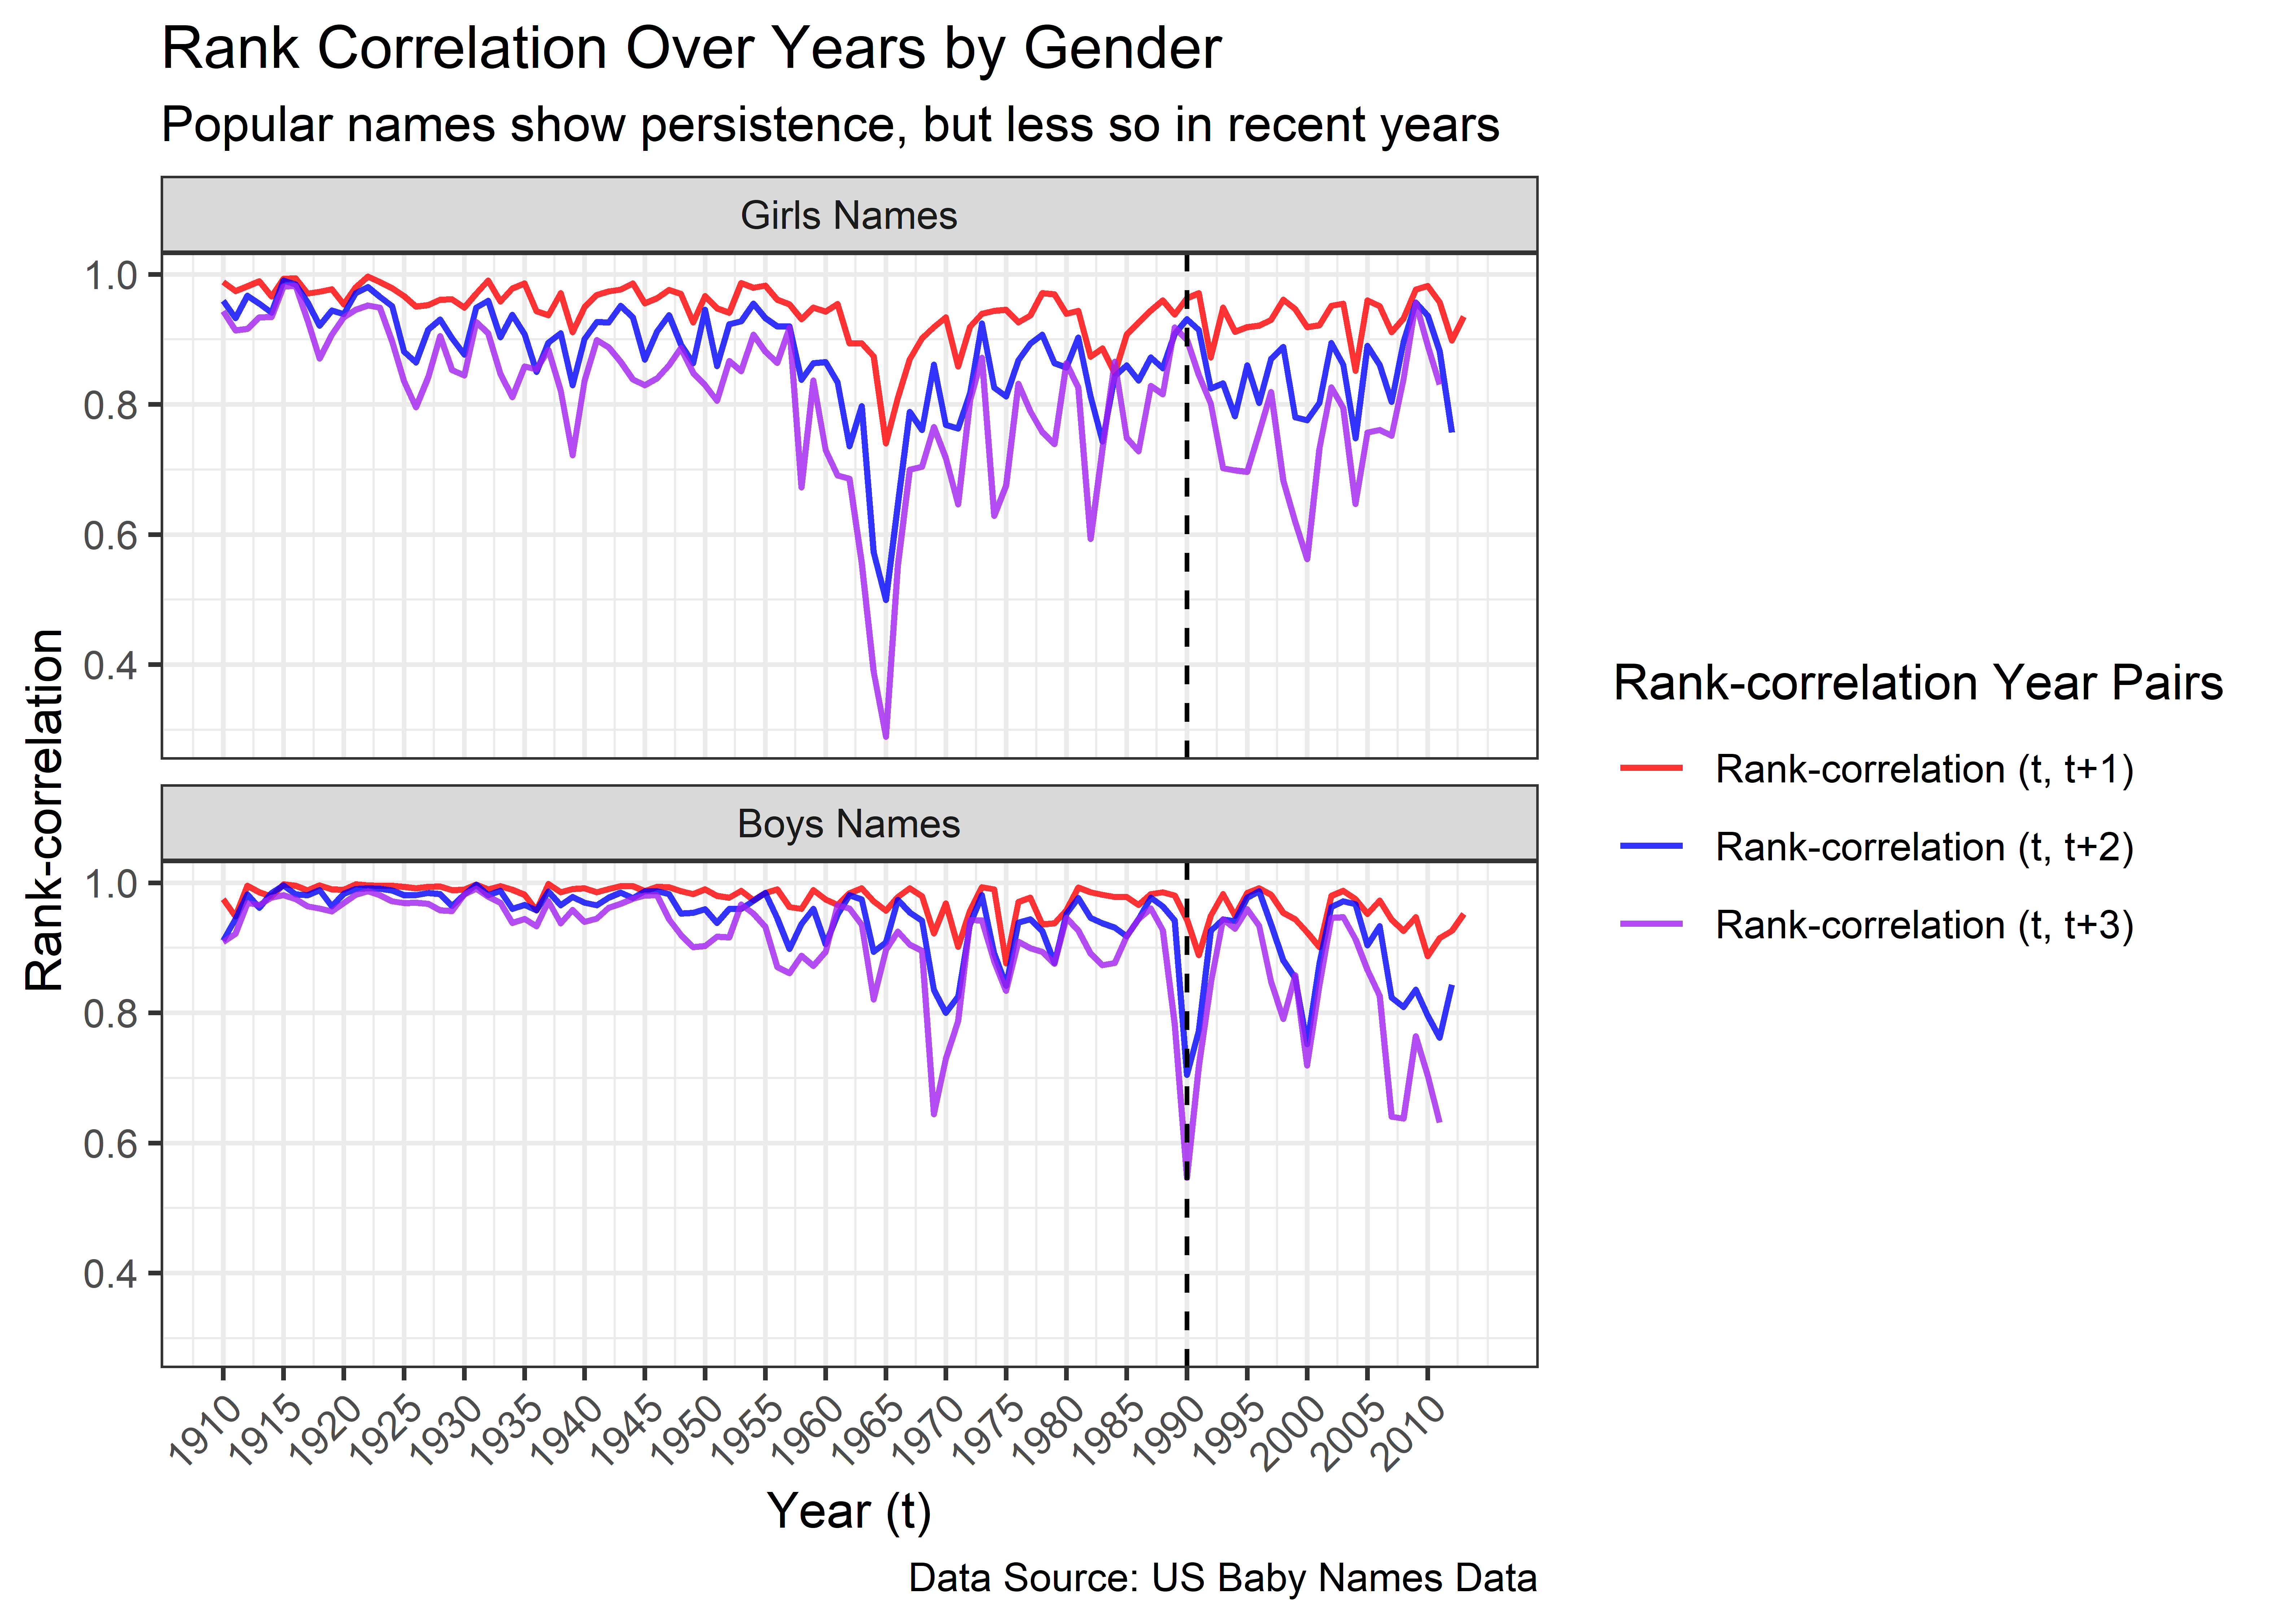
\includegraphics{Question_1_files/figure-latex/Figure1-1} 

}

\caption{Persistence of Popular Names \label{Figure1}}\label{fig:Figure1}
\end{figure}

\newpage

\hypertarget{which-names-have-surged-in-which-decades-and-why}{%
\section{\texorpdfstring{Which names have surged, in which decades and
why?
\label{surge}}{Which names have surged, in which decades and why? }}\label{which-names-have-surged-in-which-decades-and-why}}

The plots, which are shown below, highlight surges in name popularity
across certain decades. The size of the dot reflects the popularity of
the name, with the growth or fall in size being of interest. The names
were selected based on which 30 names had the highest year-on-year
growth in popularity.

\begin{itemize}
\item
  In the girls plot, Figure \ref{Figure2} below, it is evident that the
  name Jennifer and Amy spike in the 1970s, while Lisa spikes in the
  1960s and Sarah spikes in the 1980s.
\item
  Figure \ref{Figure3}, the boys name plot, shows that the names Joshua
  and Justin spike simultaneously in the 1970s and 1980s, while Jacob,
  Alexander and Nicholas grow in popularity from the 1980s.
\end{itemize}

\begin{figure}[H]

{\centering 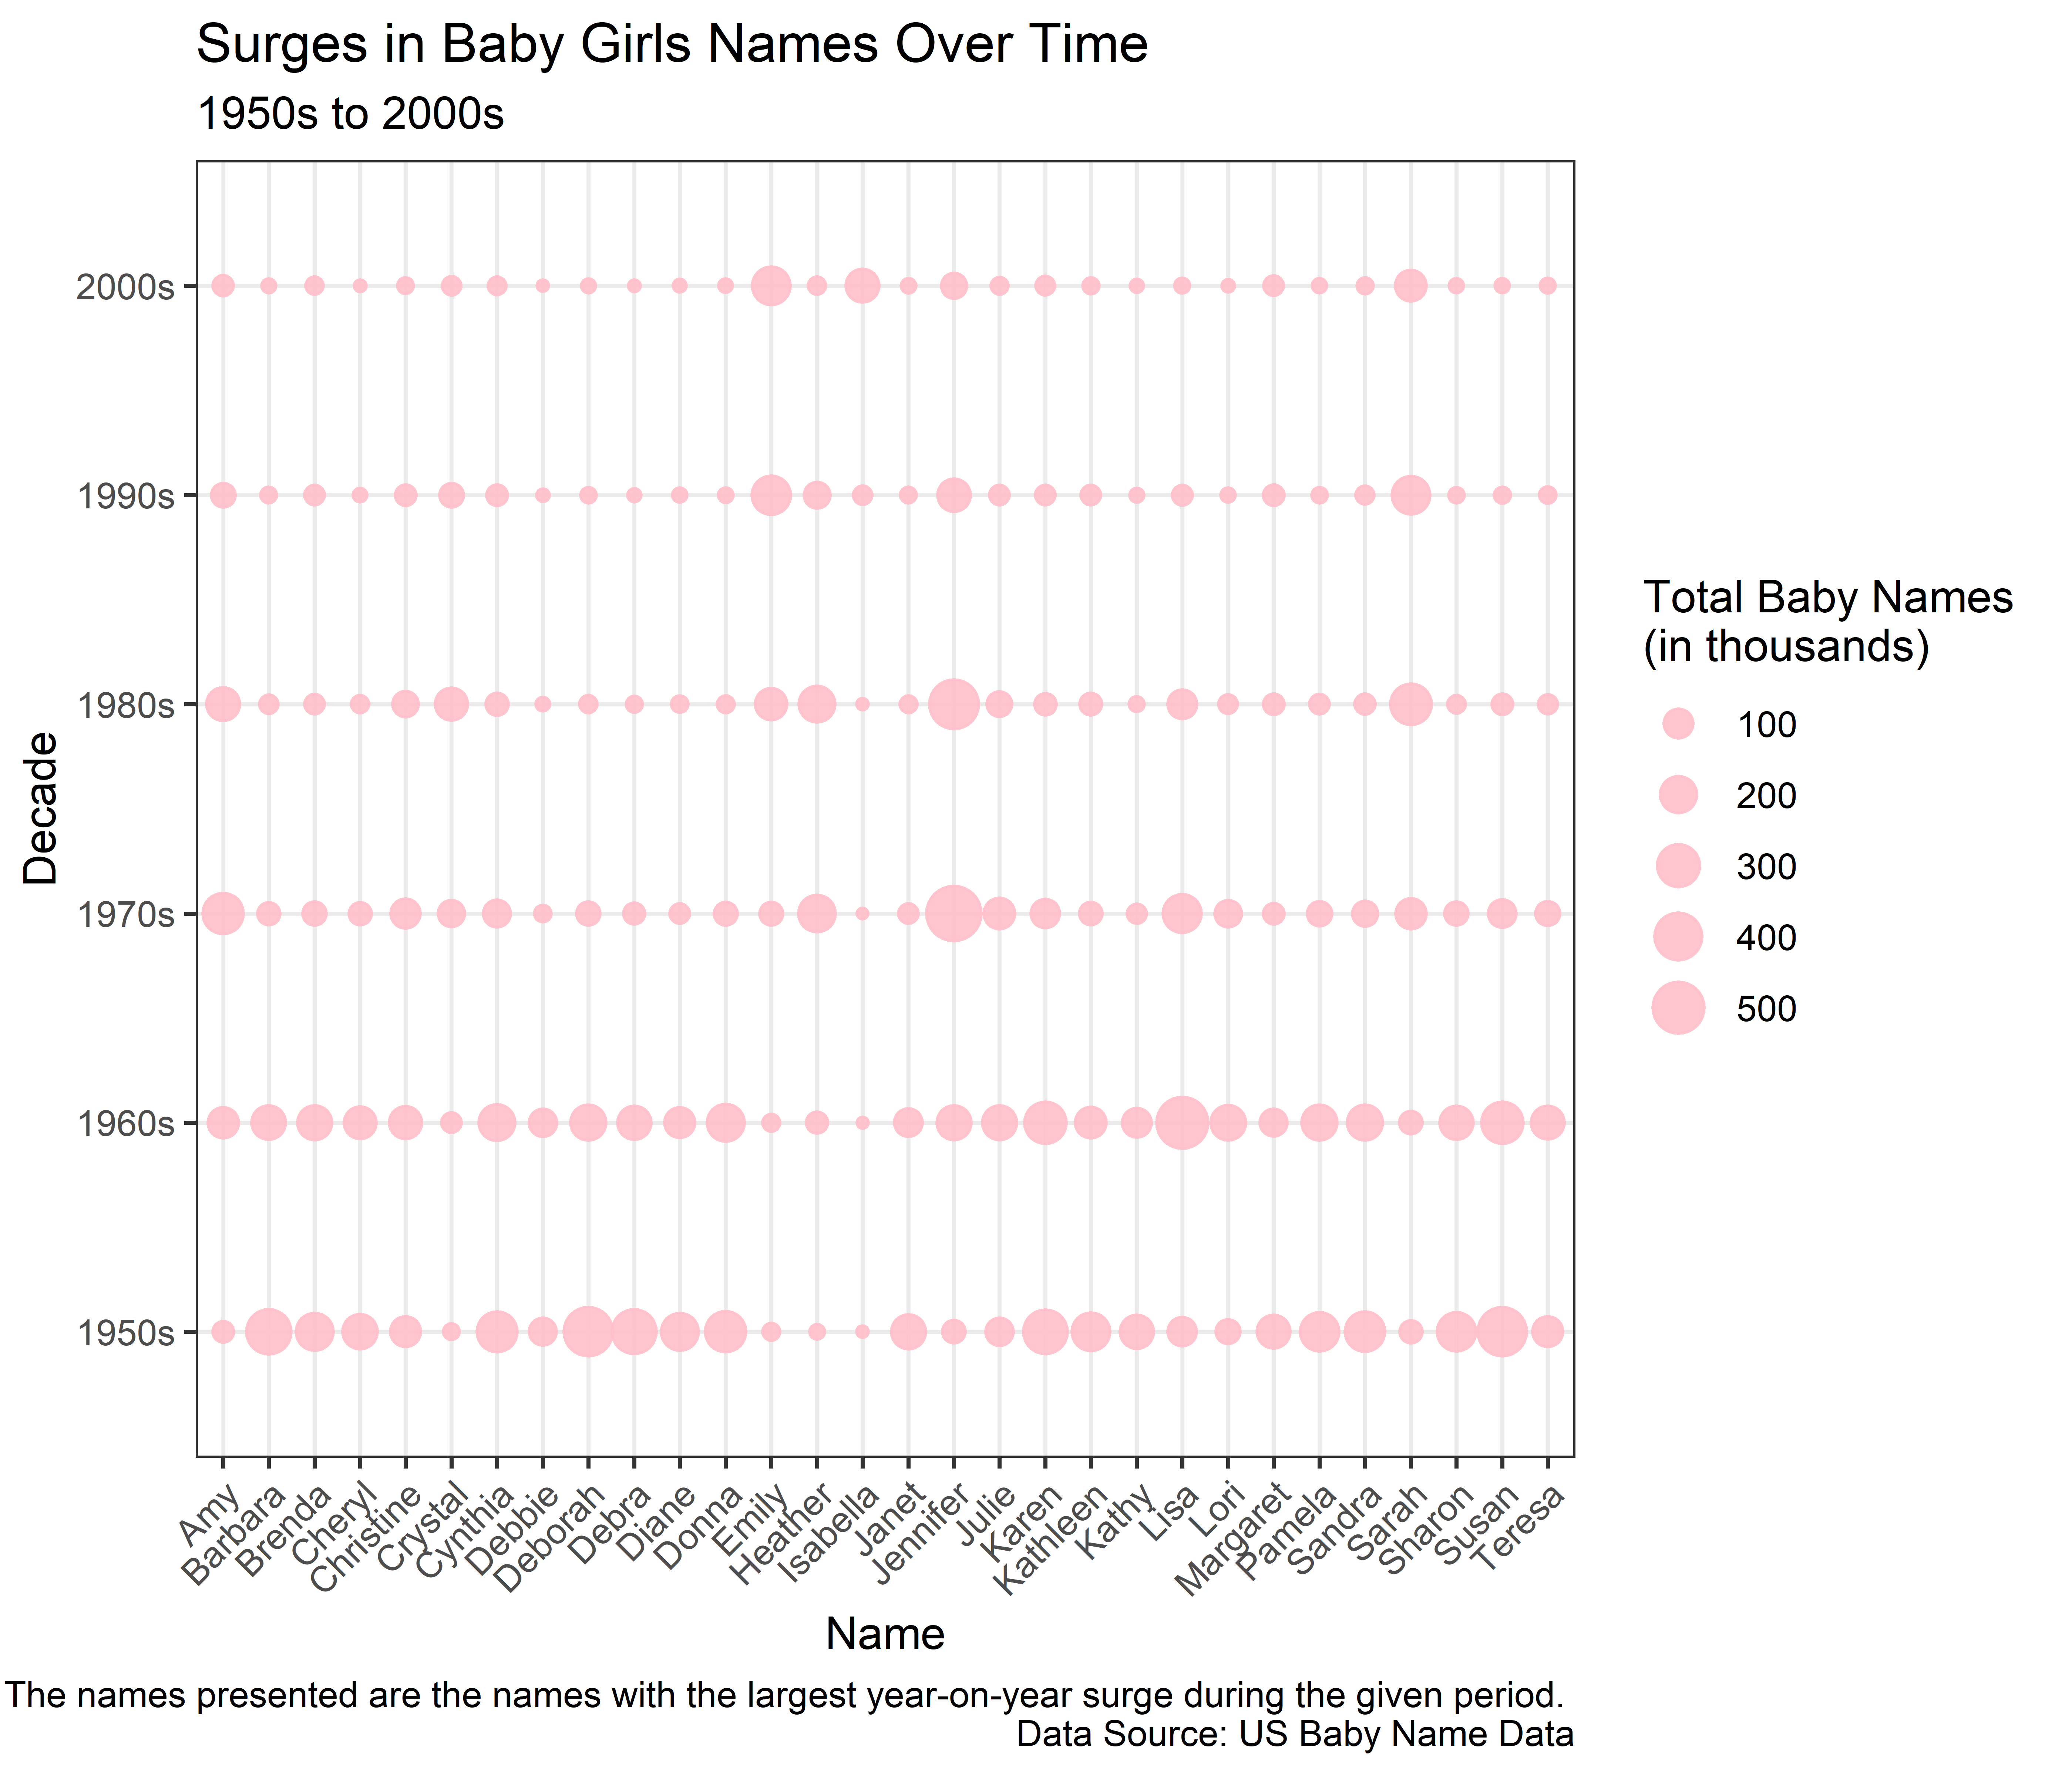
\includegraphics{Question_1_files/figure-latex/Figure2-1} 

}

\caption{Surge in Girls Names \label{Figure2}}\label{fig:Figure2}
\end{figure}

\begin{figure}[H]

{\centering 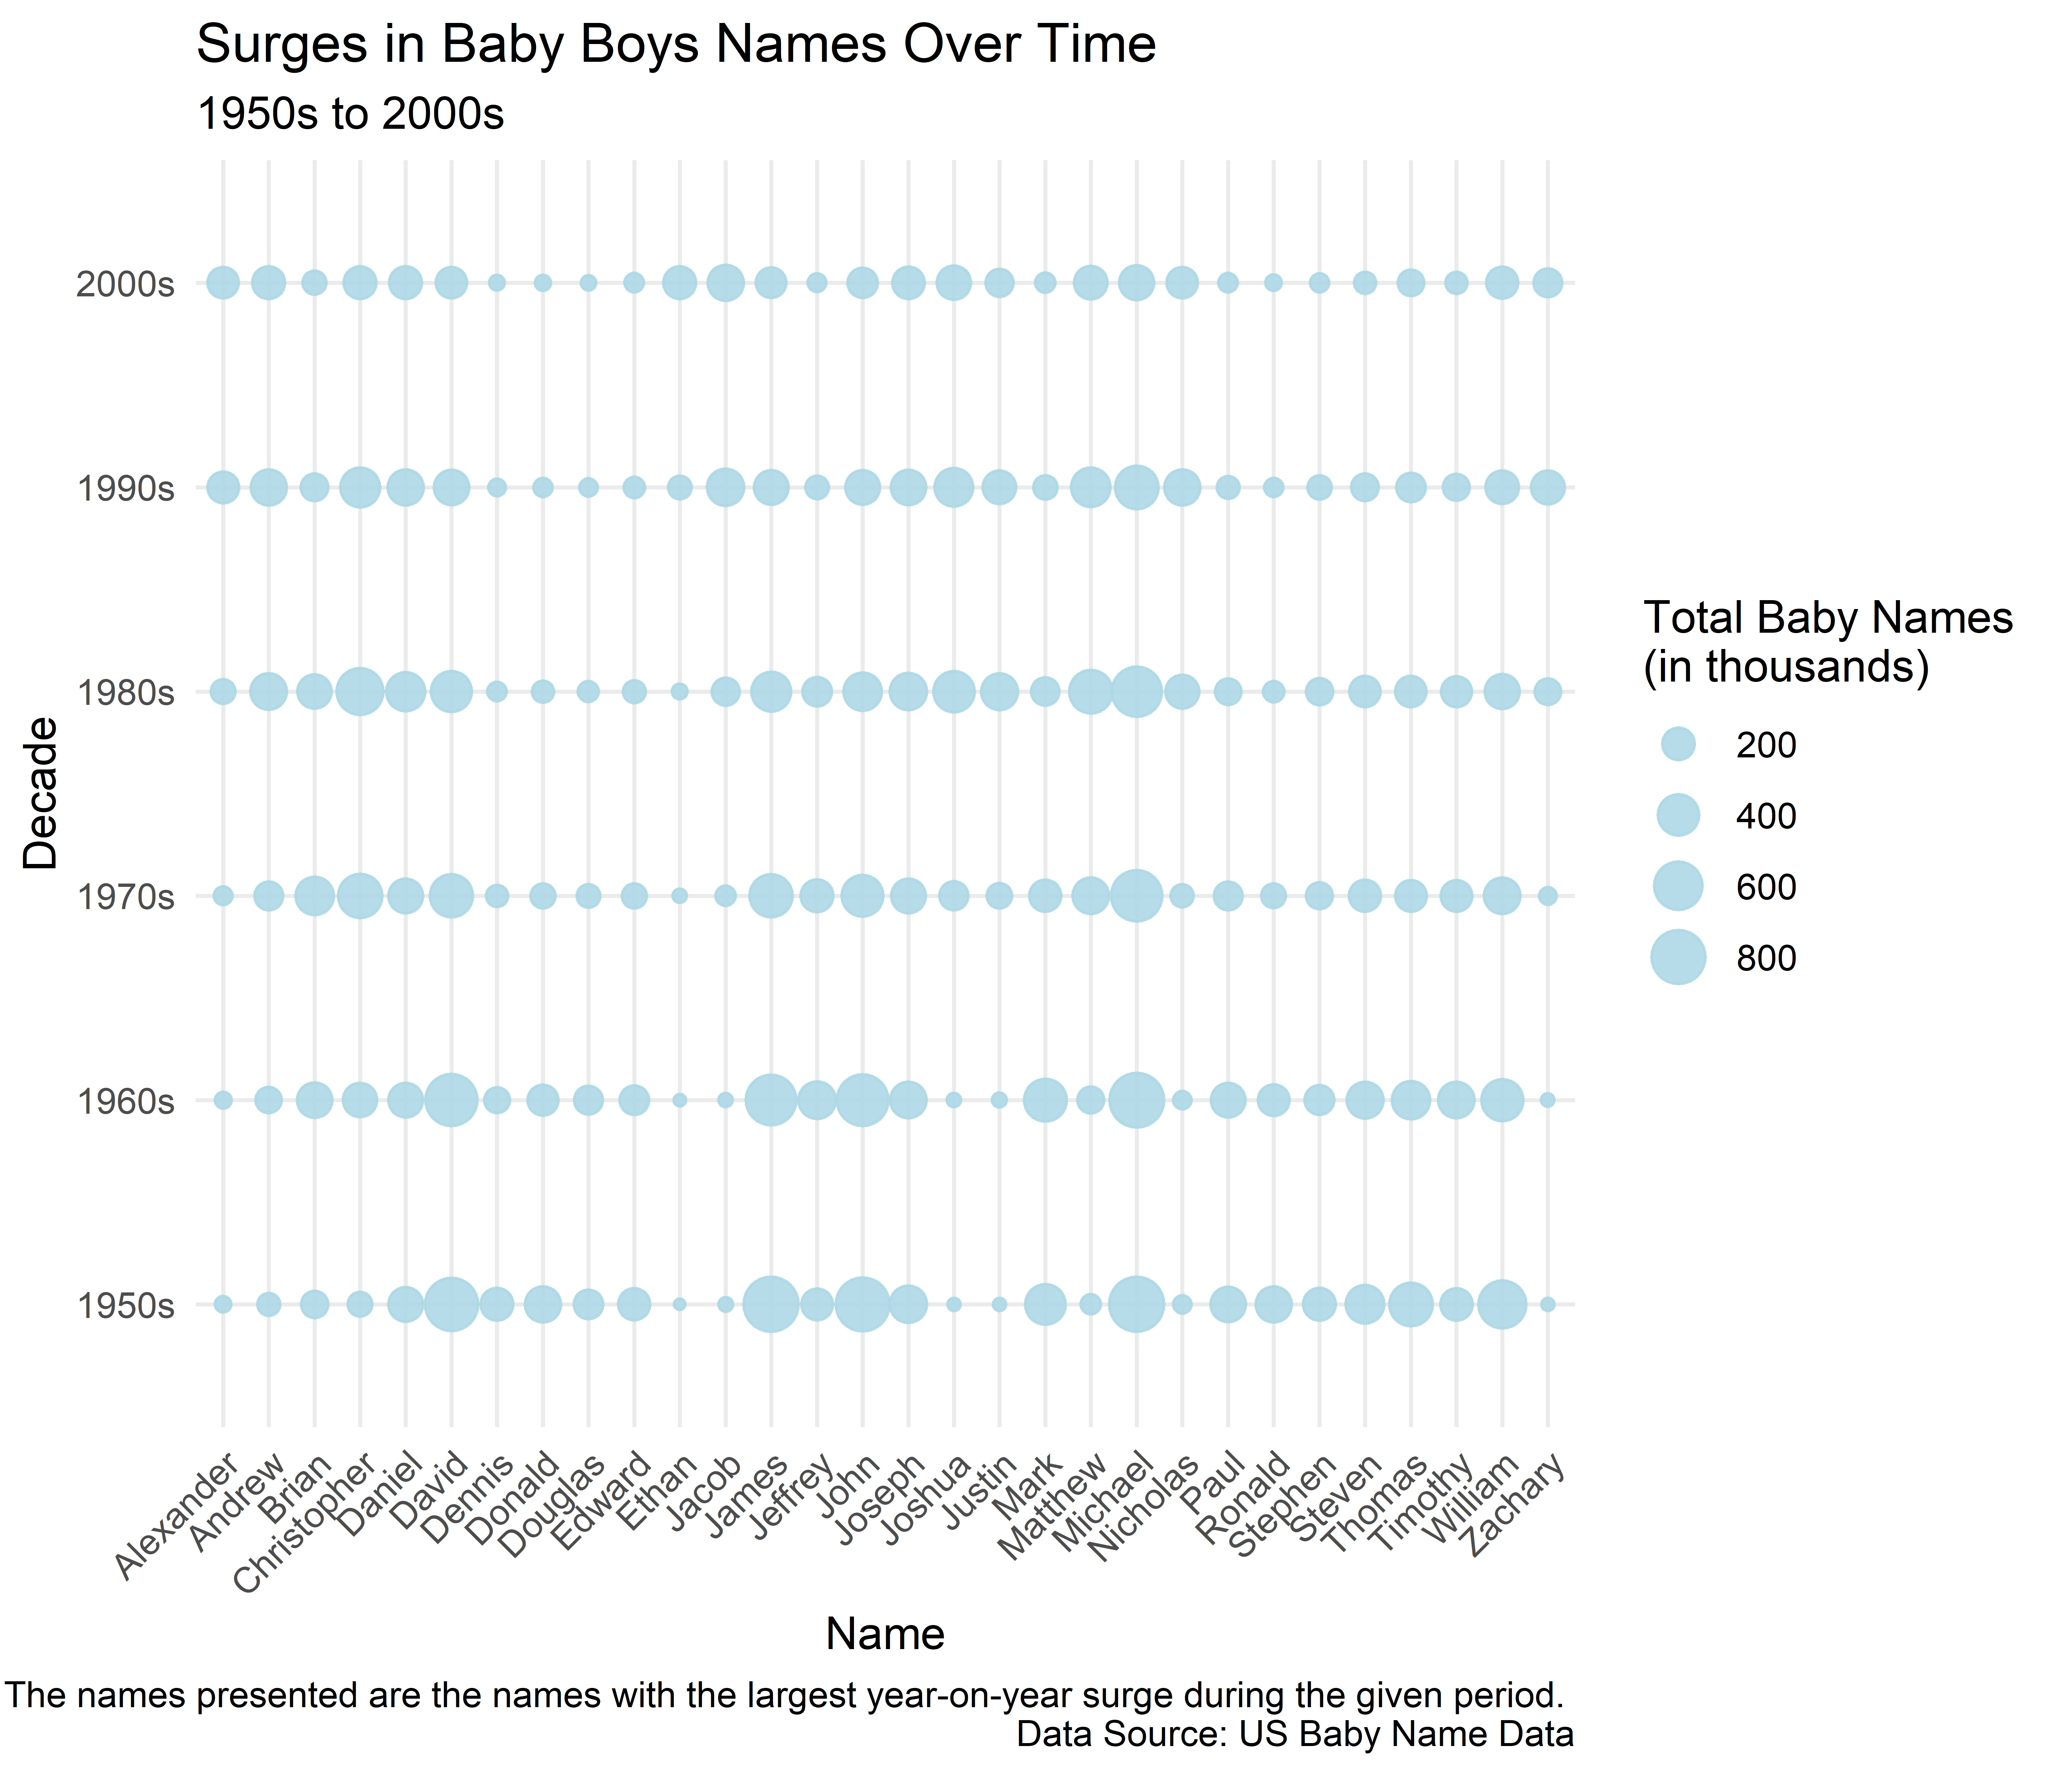
\includegraphics{Question_1_files/figure-latex/Figure3-1} 

}

\caption{Surges in Boys Names \label{Figure3}}\label{fig:Figure3}
\end{figure}

\hypertarget{notes}{%
\section{Notes}\label{notes}}

This paper was made using the Texevier
(\protect\hyperlink{ref-Texevier}{Katzke, 2017}) package.

\newpage

\hypertarget{references}{%
\section*{References}\label{references}}
\addcontentsline{toc}{section}{References}

\hypertarget{refs}{}
\begin{CSLReferences}{1}{0}
\leavevmode\vadjust pre{\hypertarget{ref-Texevier}{}}%
Katzke, N.F. 2017. \emph{{Texevier}: {P}ackage to create elsevier
templates for rmarkdown}. Stellenbosch, South Africa: Bureau for
Economic Research.

\end{CSLReferences}

\bibliography{Tex/ref}





\end{document}
